\documentclass{beamer}
\usepackage[utf8]{inputenc}
% \usepackage{default}
% \usepackage{paralist}
% \usepackage{enumitem}
\usepackage{changepage}
\usepackage{enumerate}
% \setlist{align=left}
\usetheme{Antibes}
\geometry{paper=a4}

\title{PATENA: an algorithm for the design of protein linker sequences}
% \date{5 Junio - 2015}

\begin{document}

\begin{frame}
 \titlepage
\end{frame}

\section{Intro}

\begin{frame}{Chimeric proteins}
% Very simple idea, very wide range of applications

% QUE SON
% ejemplos:
% 	Formación de proteinas bifuncionales mediante union covalente de dominios.
% 	Promover la unión entre proteinas que forman complejos, generando una unión covalente entre ellos
% 
% proceso de sintesis:
% 	-unir los dominios de interes
%       -clone into expression system

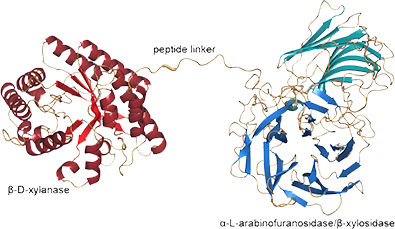
\includegraphics[width=200px]{../img/fusionEnzymes.png}
\end{frame}




\begin{frame}{Chimeric proteins}
What we need:
\begin{itemize}
 \item 2+ Globular domains
 \item Linker sequence
%  por que es necesario???
% The construction of a multifunctional enzyme by simple head-to-tail fusion of parental  enzymes  often  results  in  non-functional  enzymes
% because of either incorrect folding or restrained ability to interact with other protein subunits (Hua et al., 2004)
 \begin{itemize}
    \pause
    \item Allows domains to fold correctly, move and interact freely
%  \subitem Keep domains together so they work as a unit
\end{itemize}
\end{itemize}
% 
\includegraphics[width=10px]{../img/okMark.png}
% \hspace*{100px}
\vspace{20px}
% 
\includegraphics[width=10px]{../img/xMark.png}
\pause
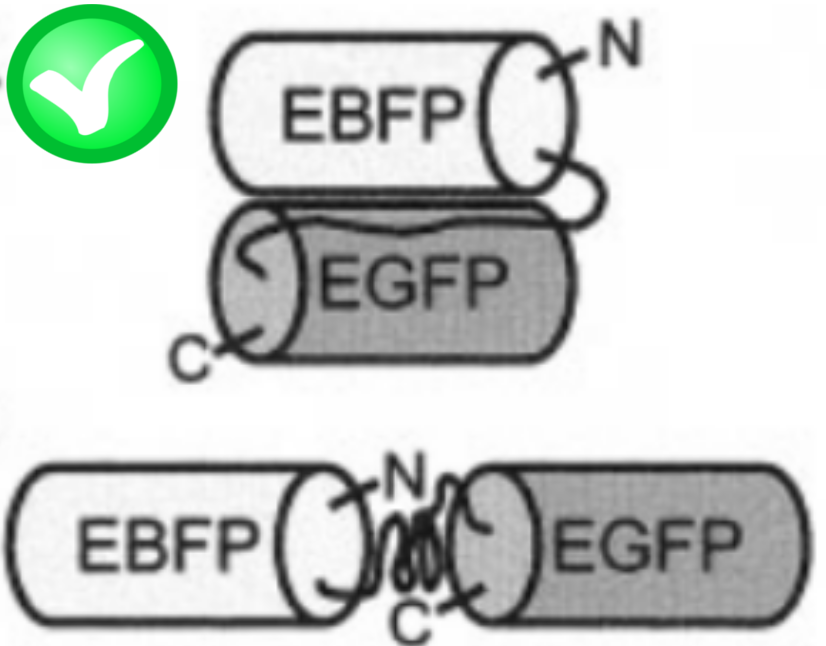
\includegraphics[width=100px]{../img/linkerOk-sign.png}
\hspace{40px}
\pause
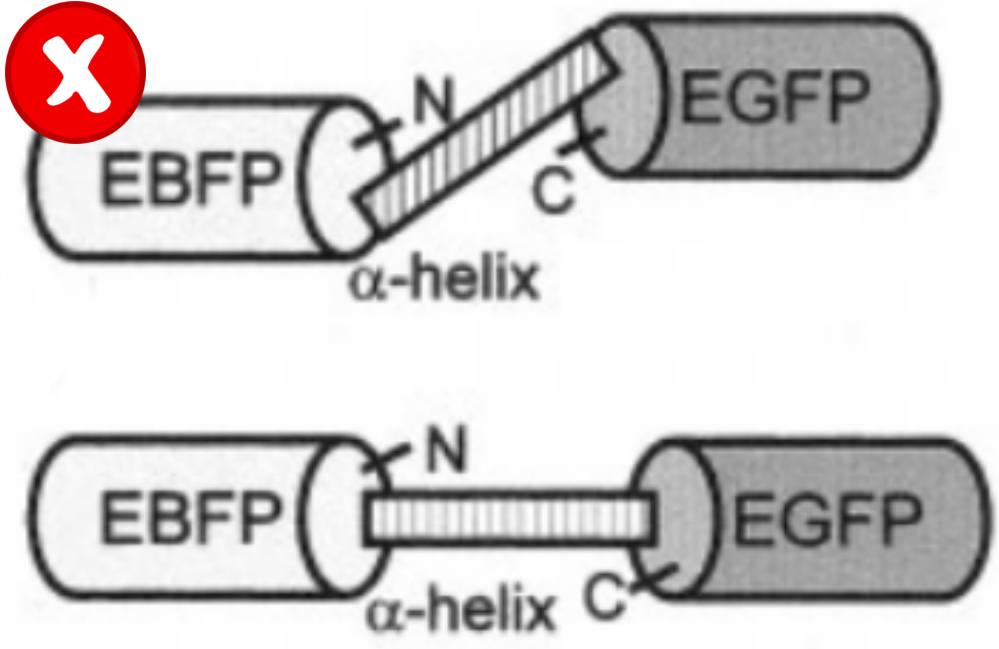
\includegraphics[width=120px]{../img/linkerBad-sign.png}
\end{frame}








\begin{frame}{Relevant linker properties}
% Based on engineering process and linker function we can extract some properties
\begin{itemize}
%   BASED ON PREVOUSLY DEFINED FUNCTION
  \item Length
  \item Intrinsically disordered
    \begin{itemize}
    \item Extended conformation
    \item Dynamic interchange
    \end{itemize}
  \item Biologically inert
  \item Composition
    \begin{itemize}
     \item AAs frequencies, UV silent, net charge
    \end{itemize}
\end{itemize}
\pause
\vspace{15px}
%  Y CON TANTOS REQUERIMIENTOS..........
\Large{....linker design is not a trivial problem}
% \pause
% \\
% \vspace{10px}
% \huge{...one solution does \textbf{NOT} fits all.}
% we need to
\end{frame}



\begin{frame}{Linker design}
% SI QUEDA MUY GRANDE ESTA DIAPO LA PUEDO DIVIDIR EN 3 PARTES....!!!
% \pause
\begin{itemize}
 \item Use natural linkers
 \pause
 \begin{itemize}
  \item structure?
  \item inert?
%  INCLUIR FIGURA!!!!

 \pause 
 \end{itemize}
 \item Intuitive design
%  there are lots of chimeric constructions that were experimentally tested....reuse. may involve small engineering process to adapt the sequence(lenght, composition, etc)
 \pause
 \begin{itemize}
  \item Reuse from literature or propose novel sequence. 
  \item Usually G/S/P-rich 
  \begin{itemize}
   \item  i.e $(GGGS)_n$) 
  \end{itemize}
  \item Very limited set of sequences and composition
  \end{itemize}
%  \pause
%  \subitem Requires experimental test (prueba y error) 

\end{itemize}
\end{frame}


\begin{frame}{Pseudo-Rational design}
%  \item Pseudo-Rational design
%   \pause 

%   \begin{itemize}
 DB (natural + literature linkers)
%  \makebox[0pt][l]{%
%   \raisebox{-\totalheight}[0pt][0pt]{%
 \hspace{10px}

\includegraphics[width=130px]{../img/synLinkerLogo.png} 
%     \includegraphics[width=4in]{book}
% }}%
 %  gives an idea of 'design', instead it is just a parametrized search. 
%  \item We cannot always get a solution %a suitable solution
\pause
% \end{itemize}

 \vspace{10px}
 \centering
  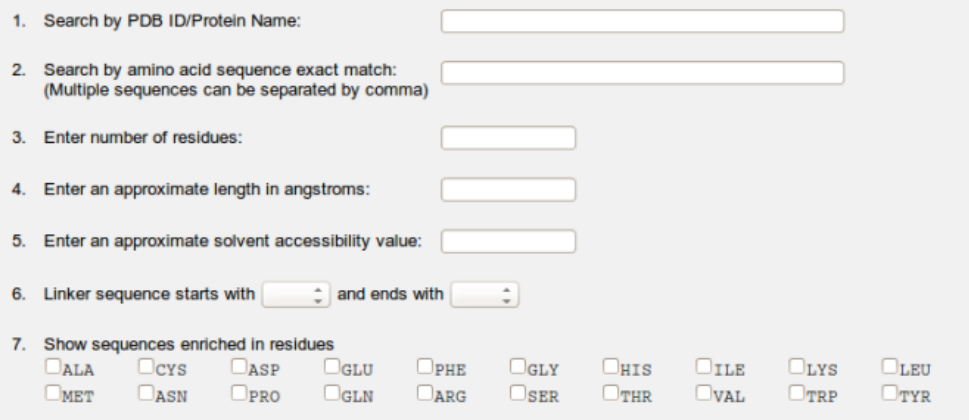
\includegraphics[width=300px]{../img/synLinker.png} 
\begin{itemize}
 \item Always applicable?
\end{itemize}

\end{frame}









\section{Method}

\begin{frame}{Rational approach}
No design method can fulfill all properties

If we have a candidate linker sequence...\\
% We can predict all wanted/unwanted properties.
% HERE I DESCRIBE THE EVALUATION OF
Disorder $\rightarrow$  IUPred \\
Inert $\rightarrow$ BLAST search, linear motifs, recognition elements\\
Aggregation propensity $\rightarrow$ TANGO\\

We can evaluate (get an idea, get an estimation of) how good or how bad(quality) is a sequence to work as a linker.
% ademas, podemos hacerlo at residue level
% es decir, para cada posicion 


% ESTO ES BASICAMENTE EL FUNDAMENTO DEL MÉTODO
% if we want to use this aspects to evaluate
% para usar esta informacion necesitamos 2 cosas
% 1 - formalize this estimation idea...i mean, we can get automatize and quantify the evaluation 
% AND
% 2 - find a good way to search for candidate sequences , to evaluate if they have the desired properties.
%	 we (probably) cant just start testing random sequences and see if they work...it would be highly inefficient
%	 we cant use natural sequences because, as we said, they dont always fulfill our needs
% 
% if we can find these 2 things we will have a design method
% 
% what is more, in our application these 2 aspects are connected !!!
\end{frame}



% ACA EXPLICO EL PUNTO 1 - CUANTIFICACION DE LA CALIDAD 
\begin{frame}{Evaluation}
%  Turn the evaluation schema into a function $f(sequence) -> score$
Turn the estimation into a scoring function...\\
Quantify how good(or bad) is a sequence
% quantify de quality of the sequence
% es decir...if we define a function f(face)
\pause
\begin{itemize}
  \item Higher score $\rightarrow$ unwanted properties $\rightarrow$ worse linker
  \item Score $\geqslant 0$ 
% we dont really care how high or low is the score, we want a linker with score = 0
\end{itemize}

% ********************
% PONER EJEMPLO DE EVALUACION, DETALLAR UN POCO MAS COMO SE HACE !!!
% EN ESTE FRAME O EN OTRO
% **************************
\end{frame}






% ACA EXPLICO EL SEGUNDO PUNTO
\begin{frame}{Search method}
% the second thing we need is 
% ahora que definimos un score

We are looking for a sequence with score = 0.
\pause

%  TENEMOS INFORMACION SOBRE DETALLADA A NIVEL DE RESIDUO(NO SOLO EL SCORE GLOBAL)
We have information of quality(score) at sequence level and residue level.
% we can use this information to guide the search

\pause
% so, we propose a search method 
We propose a search method: 
% to search for (optimal) sequence 
\begin{enumerate}
 \item Define a starting sequence 
 \item Propose point mutations to high scoring positions
%  we will get back to this later
      \begin{itemize}
      \item If score decreases $\rightarrow$ incorporate mutation to design.
      \item If it does NOT decrease score $\rightarrow$ heuristic decision.
     \end{itemize}
 \item Repeat step 2 until 

\end{enumerate}

\pause
The search(design) problem is now an optimization problem.
% and we are trying to apply an heuristic search method

% SOLVING AN OPTIMIZATION PROBLEM MIGHT HAVE DIFFERENT SOLUTIONS
% una aproximacion mediante mutaciones permitiria buscar soluciones similares a una secuencia inicial definida por el usuario
% ademas, mediante el control de la frecuencia de aminoacidos podriamos controlar la composicion

\end{frame}




\begin{frame}
\vspace{-0.5\baselineskip}
\begin{adjustwidth}{-1.5em}{-2.5em}
% \begin{adjustheight}{-1.5em}{-1.5em}
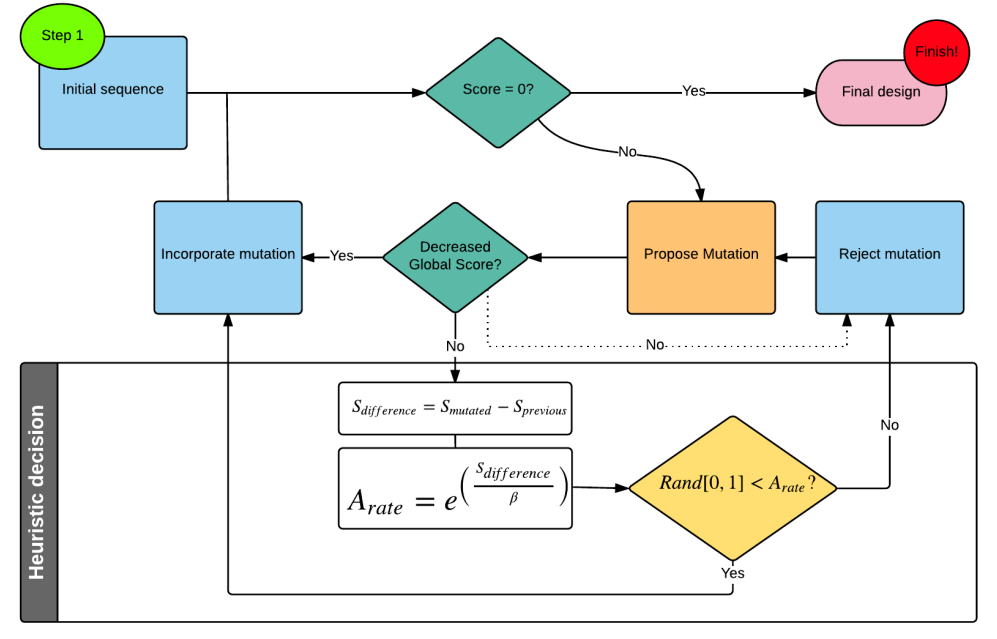
\includegraphics[width=340px,height=220px]{../img/patena2.png} 
% \end{adjustheight}
\end{adjustwidth}
% \vspace{-\baselineskip}
\end{frame}




% 
% \begin{frame}{Linkers naturales}
% No tan simples de definir/describir/clasificar
%  \begin{itemize}
%   \item Hay flexibles y rígidos    %VER MOLECULAR RULERS
%   \item Función extra: mutaciones/deleciones pueden suprimir la actividad    %FORMAN PARTE DE LA FUNCIÓN DE LA PROTEINA O SE MANTIENEN INERTES? QUIZAS NO ESTÉN EN EL DOMINIO PERO PUEDEN AYUDAR A LA ESTRUCTURA, A UNIR LIGANDOS?? A QUE MAS??
% %   PUEDE MOSTRAR UNA FUNCION EN UN CIERTO CONTEXTO EXPERIMENTAL DISTINTO AL NATURAL !!!!  
%   \end{itemize}
%  
% \end{frame}
% 



% \end{frame}
% \begin{frame}{Herramientas disponibles para elegir linkers}

% \begin{frame}{Fundamentos}
%  \begin{itemize}
%   \item Existen diversas herramientas disponibles para evaluar propiedades estructurales y funcionales a partir de la secuencia.
%   \item Existe un valor target para estas herramientas 
%   \item El número de secuencias favorables es considerablemente 'amplio' con respecto al espacio de posibles soluciones.
%  \end{itemize}
% %  La solución es una secuencia tal que las herramientas de evaluación predigan propiedades inertes y no estructuradas.
% \end{frame}




% ACLARAR QUE TODAS LAS HERRAMIENTAS SE BASAN EN LA BÚSQUEDA DE PROPIEDADES EXLUSIVAMENTE A PARTIR DE LA SECUENCIA DE AAs

% \section{Esquema para buscar una solución}
% 
% \begin{frame}{Solución planteada}
% \begin{itemize}
%  \item Iniciamos la búsqueda mediante una secuencia random o definida por el usuario. Es solo un punto de partida!
%  \item Definimos un mecanismo de score por posición en función del resultado de las herramientas:
%     Menor score = mejor solución  
%  \item Mutamos y reevaluamos iterativamente la secuencia inicial, en búsqueda de score mínimo(0). 
%  \item Las mutacione son aceptadas heurísticamente siguiendo un método de Monte Carlo, guiado por el score global (suma de puntajes de todas posiciones de la secuencia).
% \end{itemize}
% \end{frame}

% \begin{frame}
%  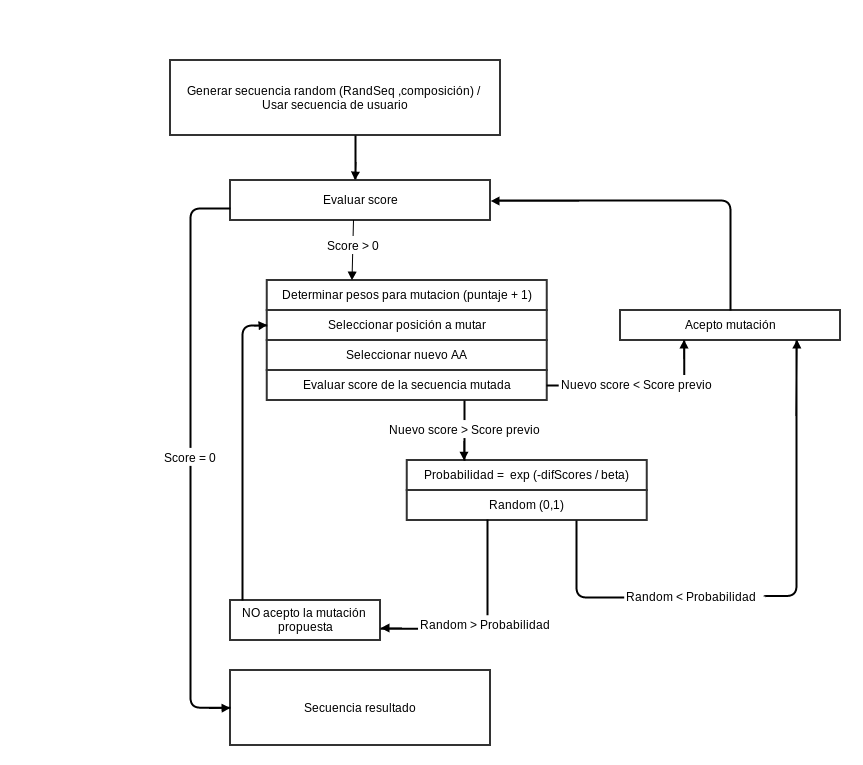
\includegraphics[width=\textwidth,height=\textheight]{esquemaGeneral.png}
% \end{frame}
% 


% \section{Herramientas de evaluación}

% % \subsection
% \begin{frame}{Herramientas ya implementadas}
% %  ESTAN SON LAS QUE YA EXPLIQUE LA VEZ PASADA
% \begin{description}[]
% %   \begin{itemize}
%    \item[IUPred:] Predicción de conformación definida 
%    \item[ANCHOR:] Predicción de proteinas que adoptan estructuras al unirse a otras. 
%    \item[BLAST:] Funcionalidad mediante homología secuencial  
%    \item[ELM:] Principales módulos funcionales encontrados en regiones intrínsecamente desordenadas.
%    \item[Prosite:] Motivos lineales que podrían estar asociados a funciones.
% %    \end{itemize}
% \end{description}
% 
% \end{frame}


% \subsection{Nuevas herramientas incorporadas}
% 
% \begin{frame}{Tango}
% El método se deriva a partir de aplicar la mecánica estadística a un conjunto de datos 
% experimentales obtenidos de los residuos en de proteinas que promueven la formacion de amyloids. 
% 
% Resulta en una probabilidad de cada residuo a adoptar cierta conformación:
% \\[2ex]
% \begin{tabular}[h]{c| c| c| c| c| c| c}
% res & aa & Beta &Turn &	Helix	& Aggregation &	Conc-Stab\_Aggregation \\
% 01 &	L	&3.5&	 0.0&	0.000&	0.000 &	0.000\\ 
% 
% \end{tabular}
% \end{frame}


% \begin{frame}{Waltz}  
%   \begin{itemize}
%    \item Determinantes secuenciales de la formación de amyloids
%    \item Utiliza una PSSM derivada de información secuencial y propiedades fisicoquímicas y estructurales. 
%   \end{itemize}
% 
% \end{frame}
% 
% \begin{frame}{Limbo}  
%   \begin{itemize}
%    \item Predice sitios de unión a chaperonas (heptapéptidos) 
%    \item Información de estudios secuenciales(ensayos de binding)
%    \item Parámetros estructurales obtenidos de modelado por homología. Structural parameters from homology modelling
%    \item Evaluación = aplicar una matriz de scores. 
%    \item Resultado=scores por posición. Importancia del threshold
%   \end{itemize}
% 
% \end{frame}

% \begin{frame}{Determinantes secuenciales para formación de Amyloids}  
%  Determinados a partir de un conjunto de péptidos cortos sintetizados y evaluados experimentalmente.
%  
%  A pH Neutral:
%  
%  ${P}_1 - {PKRHW}_2 -[VLS(C)WFNQ]_3 -[ILTYWFN]_4 - [FIY]_5- {PKRH}_6$
% \end{frame}
% 
% \begin{frame}{Secuencias transmembrana}
%  \begin{itemize}
%   \item TMHMM Server v. 2.0
%   \item Usado como clasificador binario: transmembana o no
%  \end{itemize}
% 
% \end{frame}

% 
% \begin{frame}{Pasta}
% Predicción de agregación amiloide
% \begin{itemize}
%  \item Asume que las interacciones en la formación de estructuras cross-beta(estructura asociada a fibras amiloides) es el mismo que ocurre en las estructuras de hoja plegada beta.
%  \item Utiliza un conjunto de datos de estructuras conocidas para derivar un potencial estadístico de interacción entre cada par posible de AAs en este tipo de estructura.
%  \item Durante la evaluación, el algoritmo utiliza este potencial para evaluar todos los posibles emparejamientos de la secuencia input con si misma, tanto paralela como antiparalelamente.
%  \item El emparejamiento que tenga menor energia asignada se predice como el que se adopará en caso que se forme el agregado de tipo amiloide.
% \end{itemize}
% 
%  
% \end{frame}
% % 
% \begin{frame}{Pasta}	
%  \includegraphics[width=\textwidth,height=0.9\textheight]{pastaExample.pdf}
% \end{frame}

% \begin{frame}{Pasta}	
% 
% *************************************
% Starting PASTA evaluation
% Threshold: 0.1
% Hit:
% Positions:    1-4
% RESULTS:
% M|V|L|S|P|A|D|K|T|N|V|K|A|A|W|G|K|V|G|A|H|A|G|E|Y|G|A|E
% 1|1|1|1|1|0|0|0|0|0|0|0|0|0|0|0|0|0|0|0|0|0|0|0|0|0|0|0
% Hit enter to continue with next evaluation
% 
% \end{frame}

% \subsection
% \begin{frame}{Otras funcionalidades}
%  \begin{itemize}
%   \item Carga neta de la secuencia
%   \item Secuencias flanqueantes estáticas
%   \item Distintas opciones de ejecución: full verbose,silent, limite de iteraciones, deshabilitar herramientas puntuales
%  \end{itemize}
% \end{frame}
% 
% \section{Ejemplo}
% \begin{frame}{Evaluación}
%  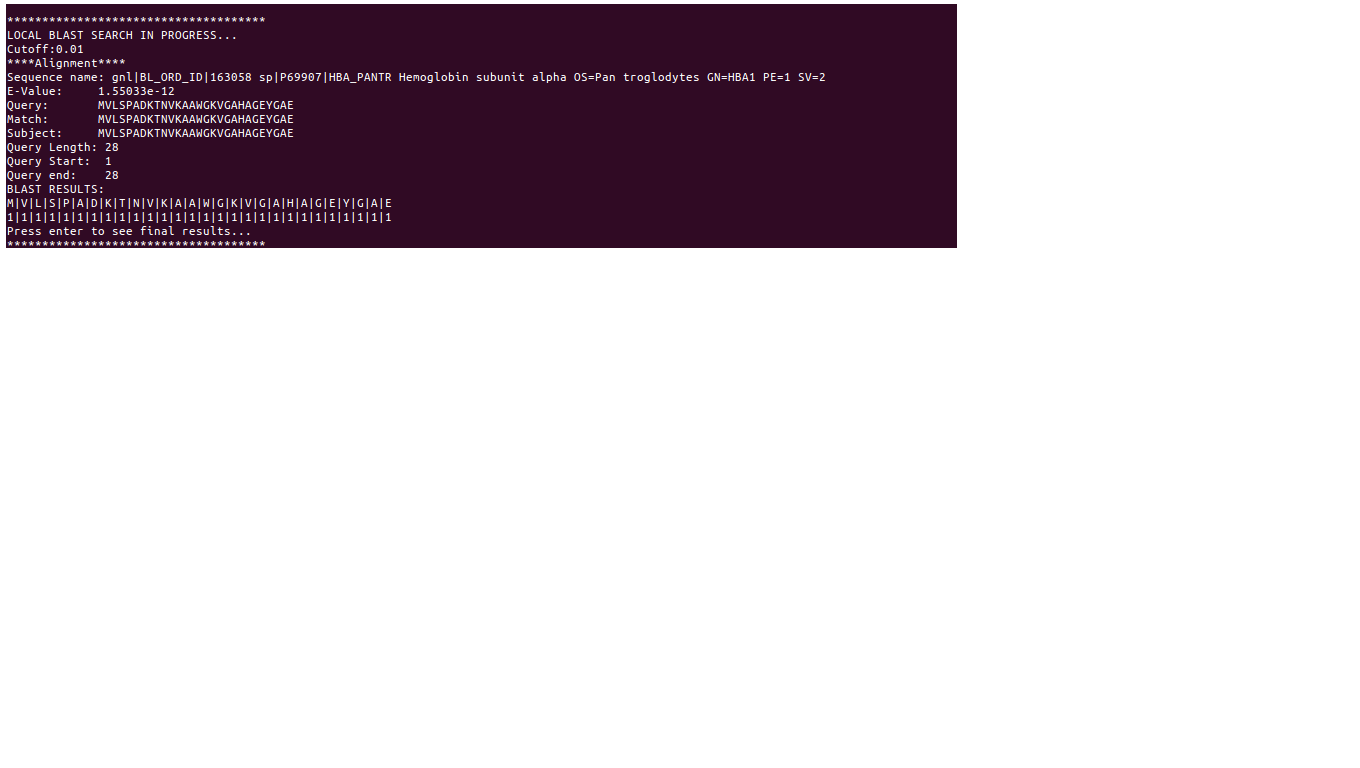
\includegraphics[width=1.7\textwidth,height=2.2\textheight]{blastExample.png}
% \end{frame}
% 
% \begin{frame}{Propuesta de mutación}
%  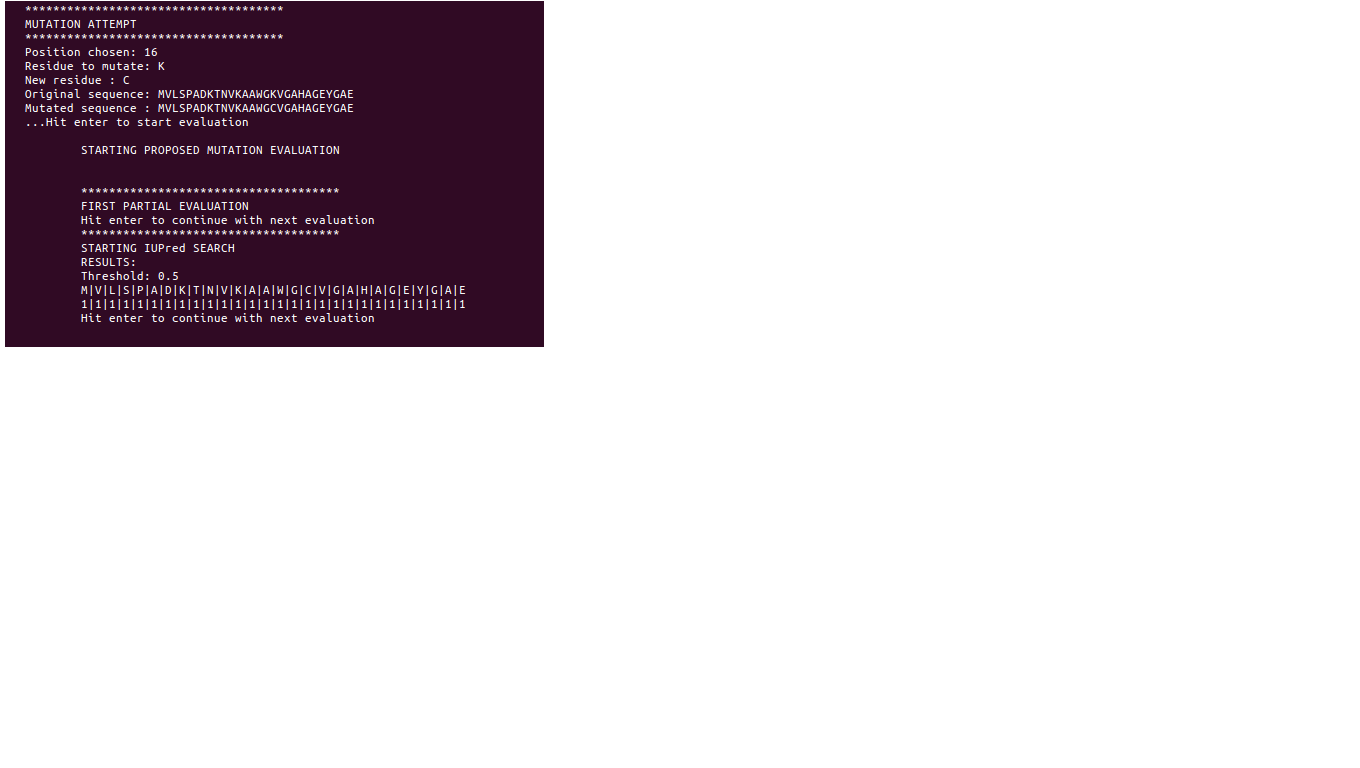
\includegraphics[width=2.4\textwidth,height=1.9\textheight]{mutAttempt.png}
% \end{frame}
% 
% \begin{frame}{Decisión}
%  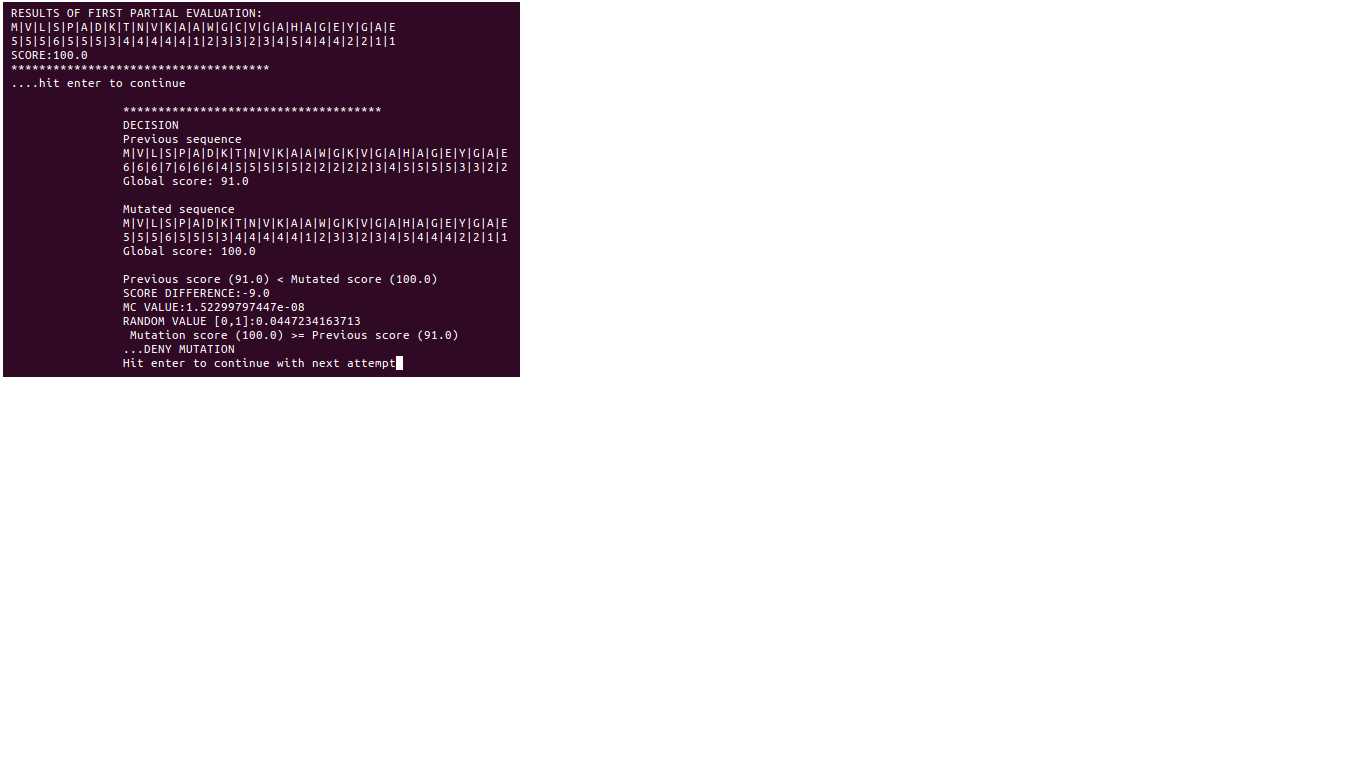
\includegraphics[width=2.4\textwidth,height=1.9\textheight]{decision.png}
% \end{frame}


% \section{Resultados}
% \begin{frame}{Tests}
 
% \end{frame}
% 
% \begin{frame}{Tiempo de ejecución - Beta = 1.0}
% 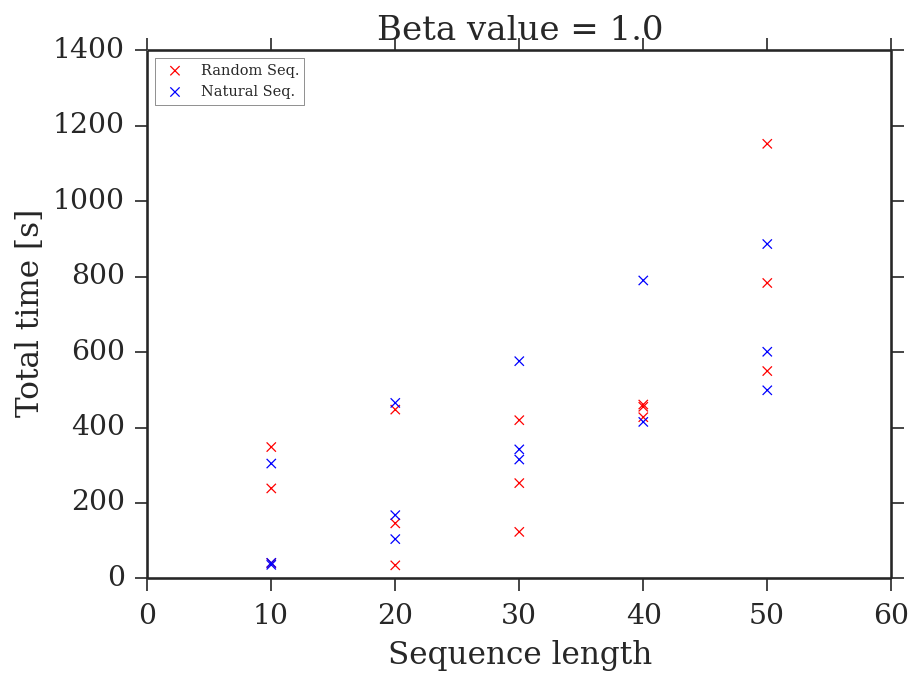
\includegraphics[width=\textwidth,height=0.8\textheight]{largo-beta.png}
% \end{frame}
% 
% 
% \begin{frame}{Tiempo de ejecución - Seq = 30}
% 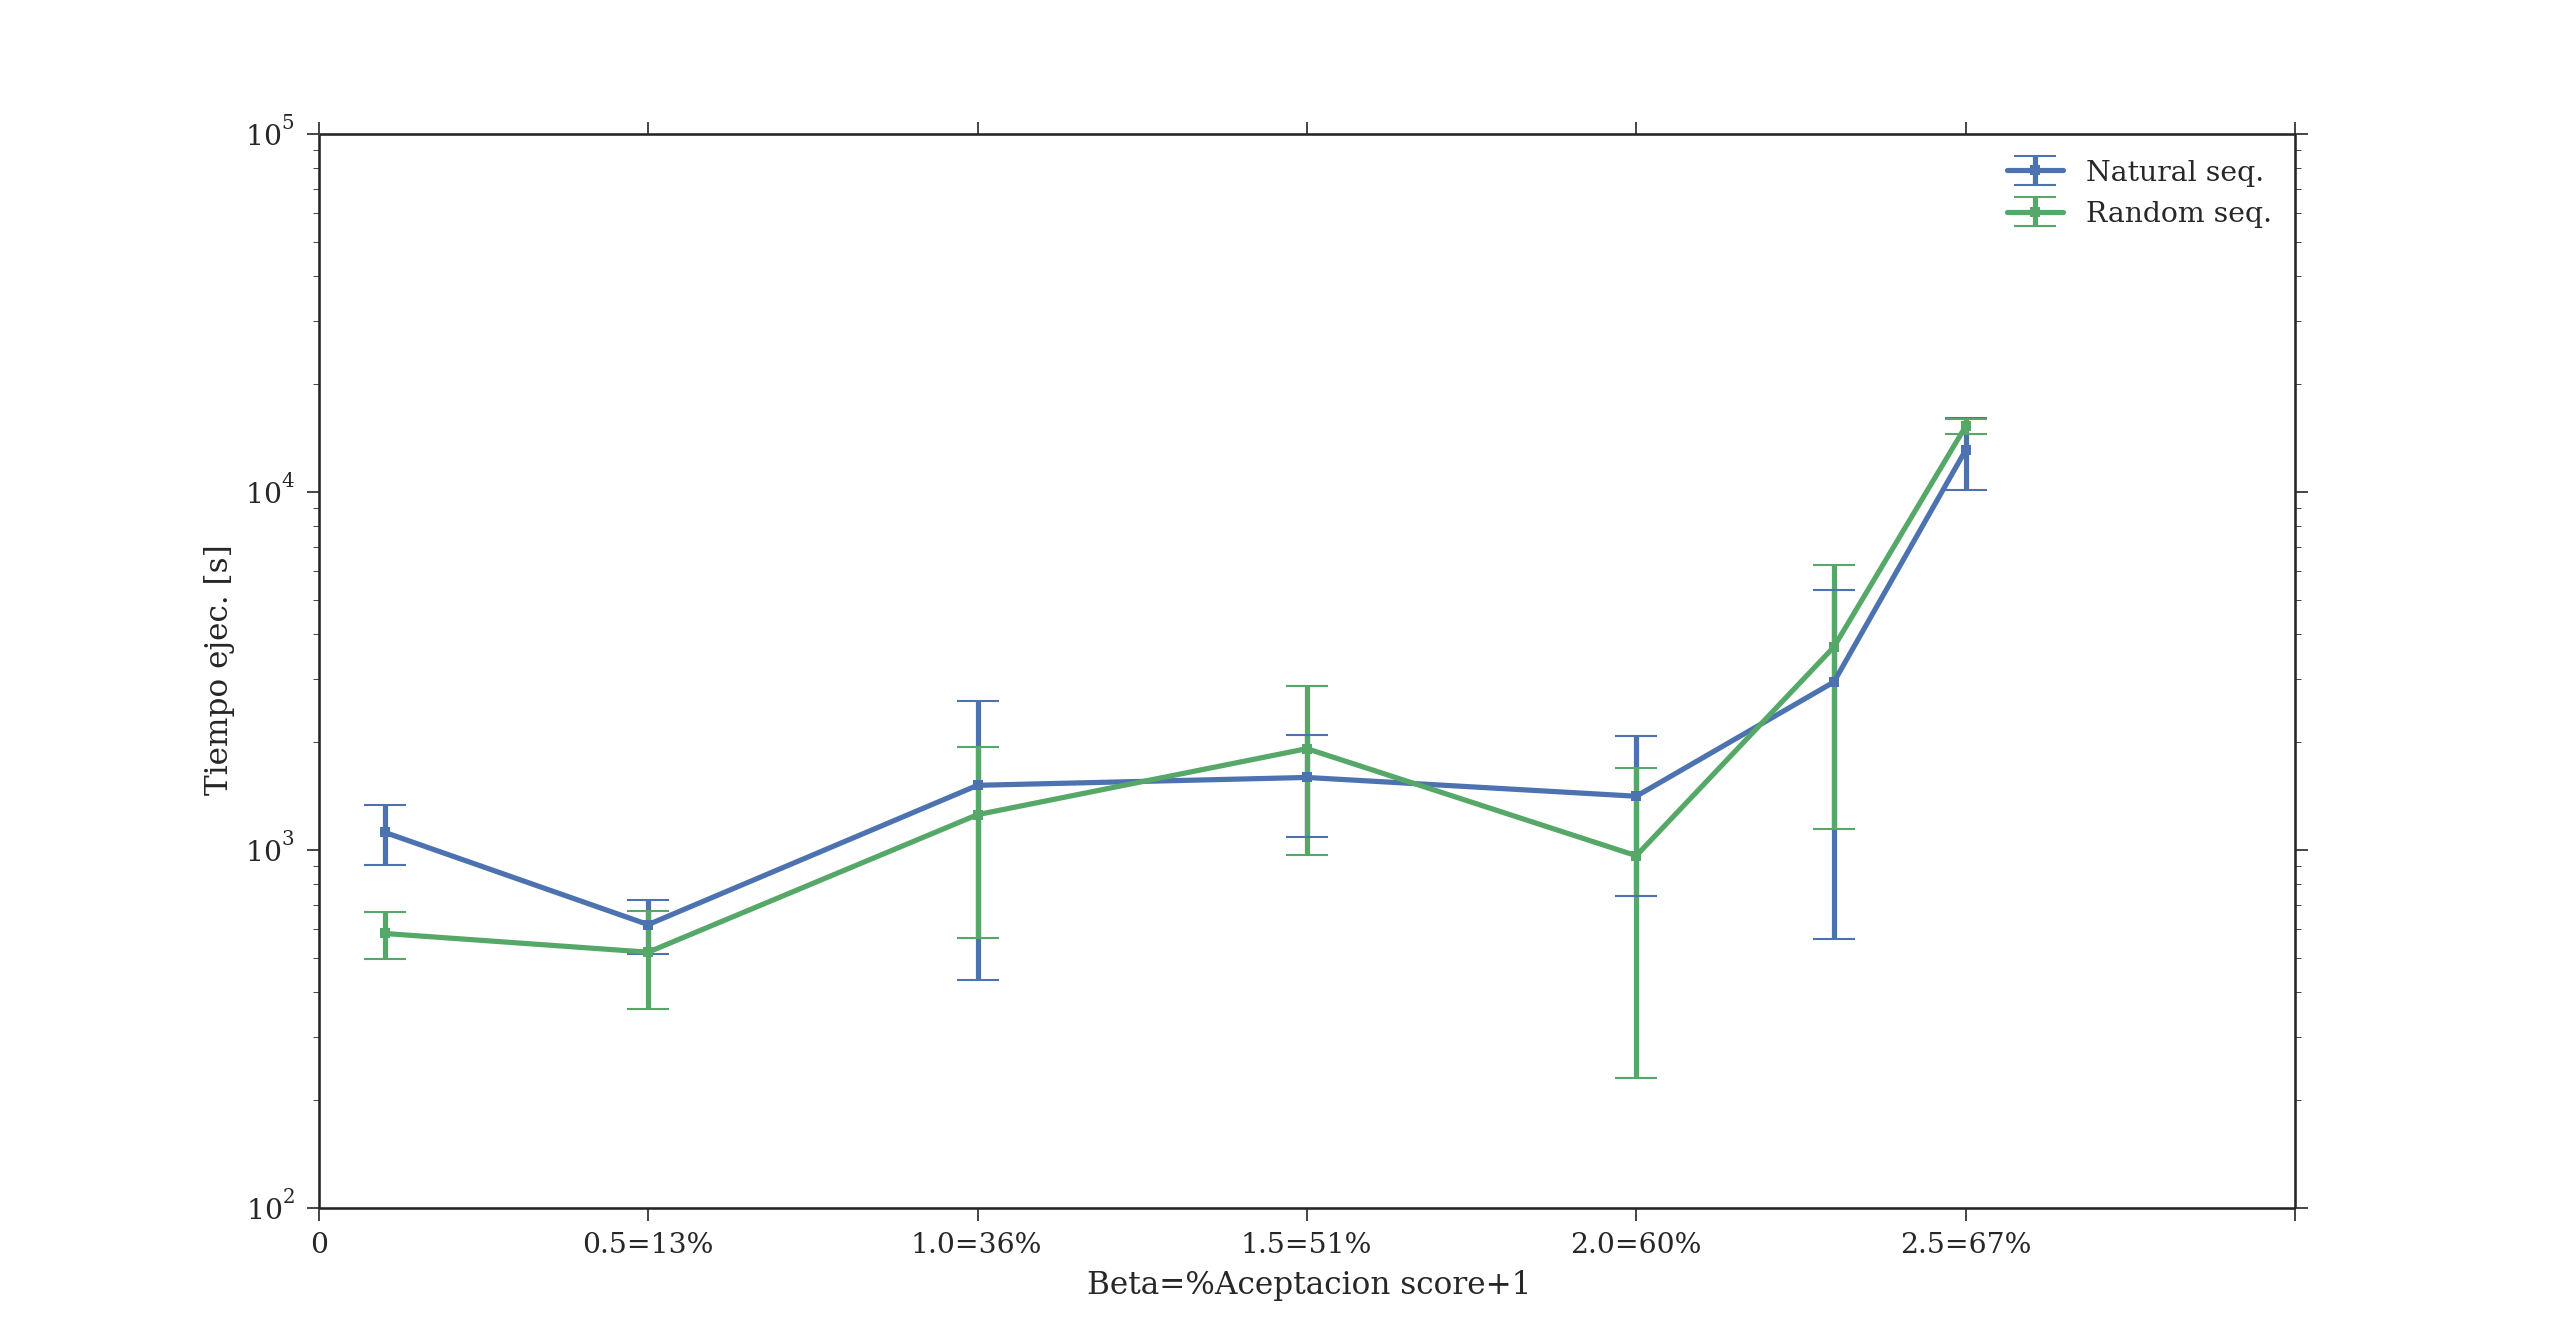
\includegraphics[width=\textwidth,height=0.85\textheight]{beta-time.png}
% \end{frame}
% 
% \begin{frame}{Intentos de mutación - Seq = 30}
% 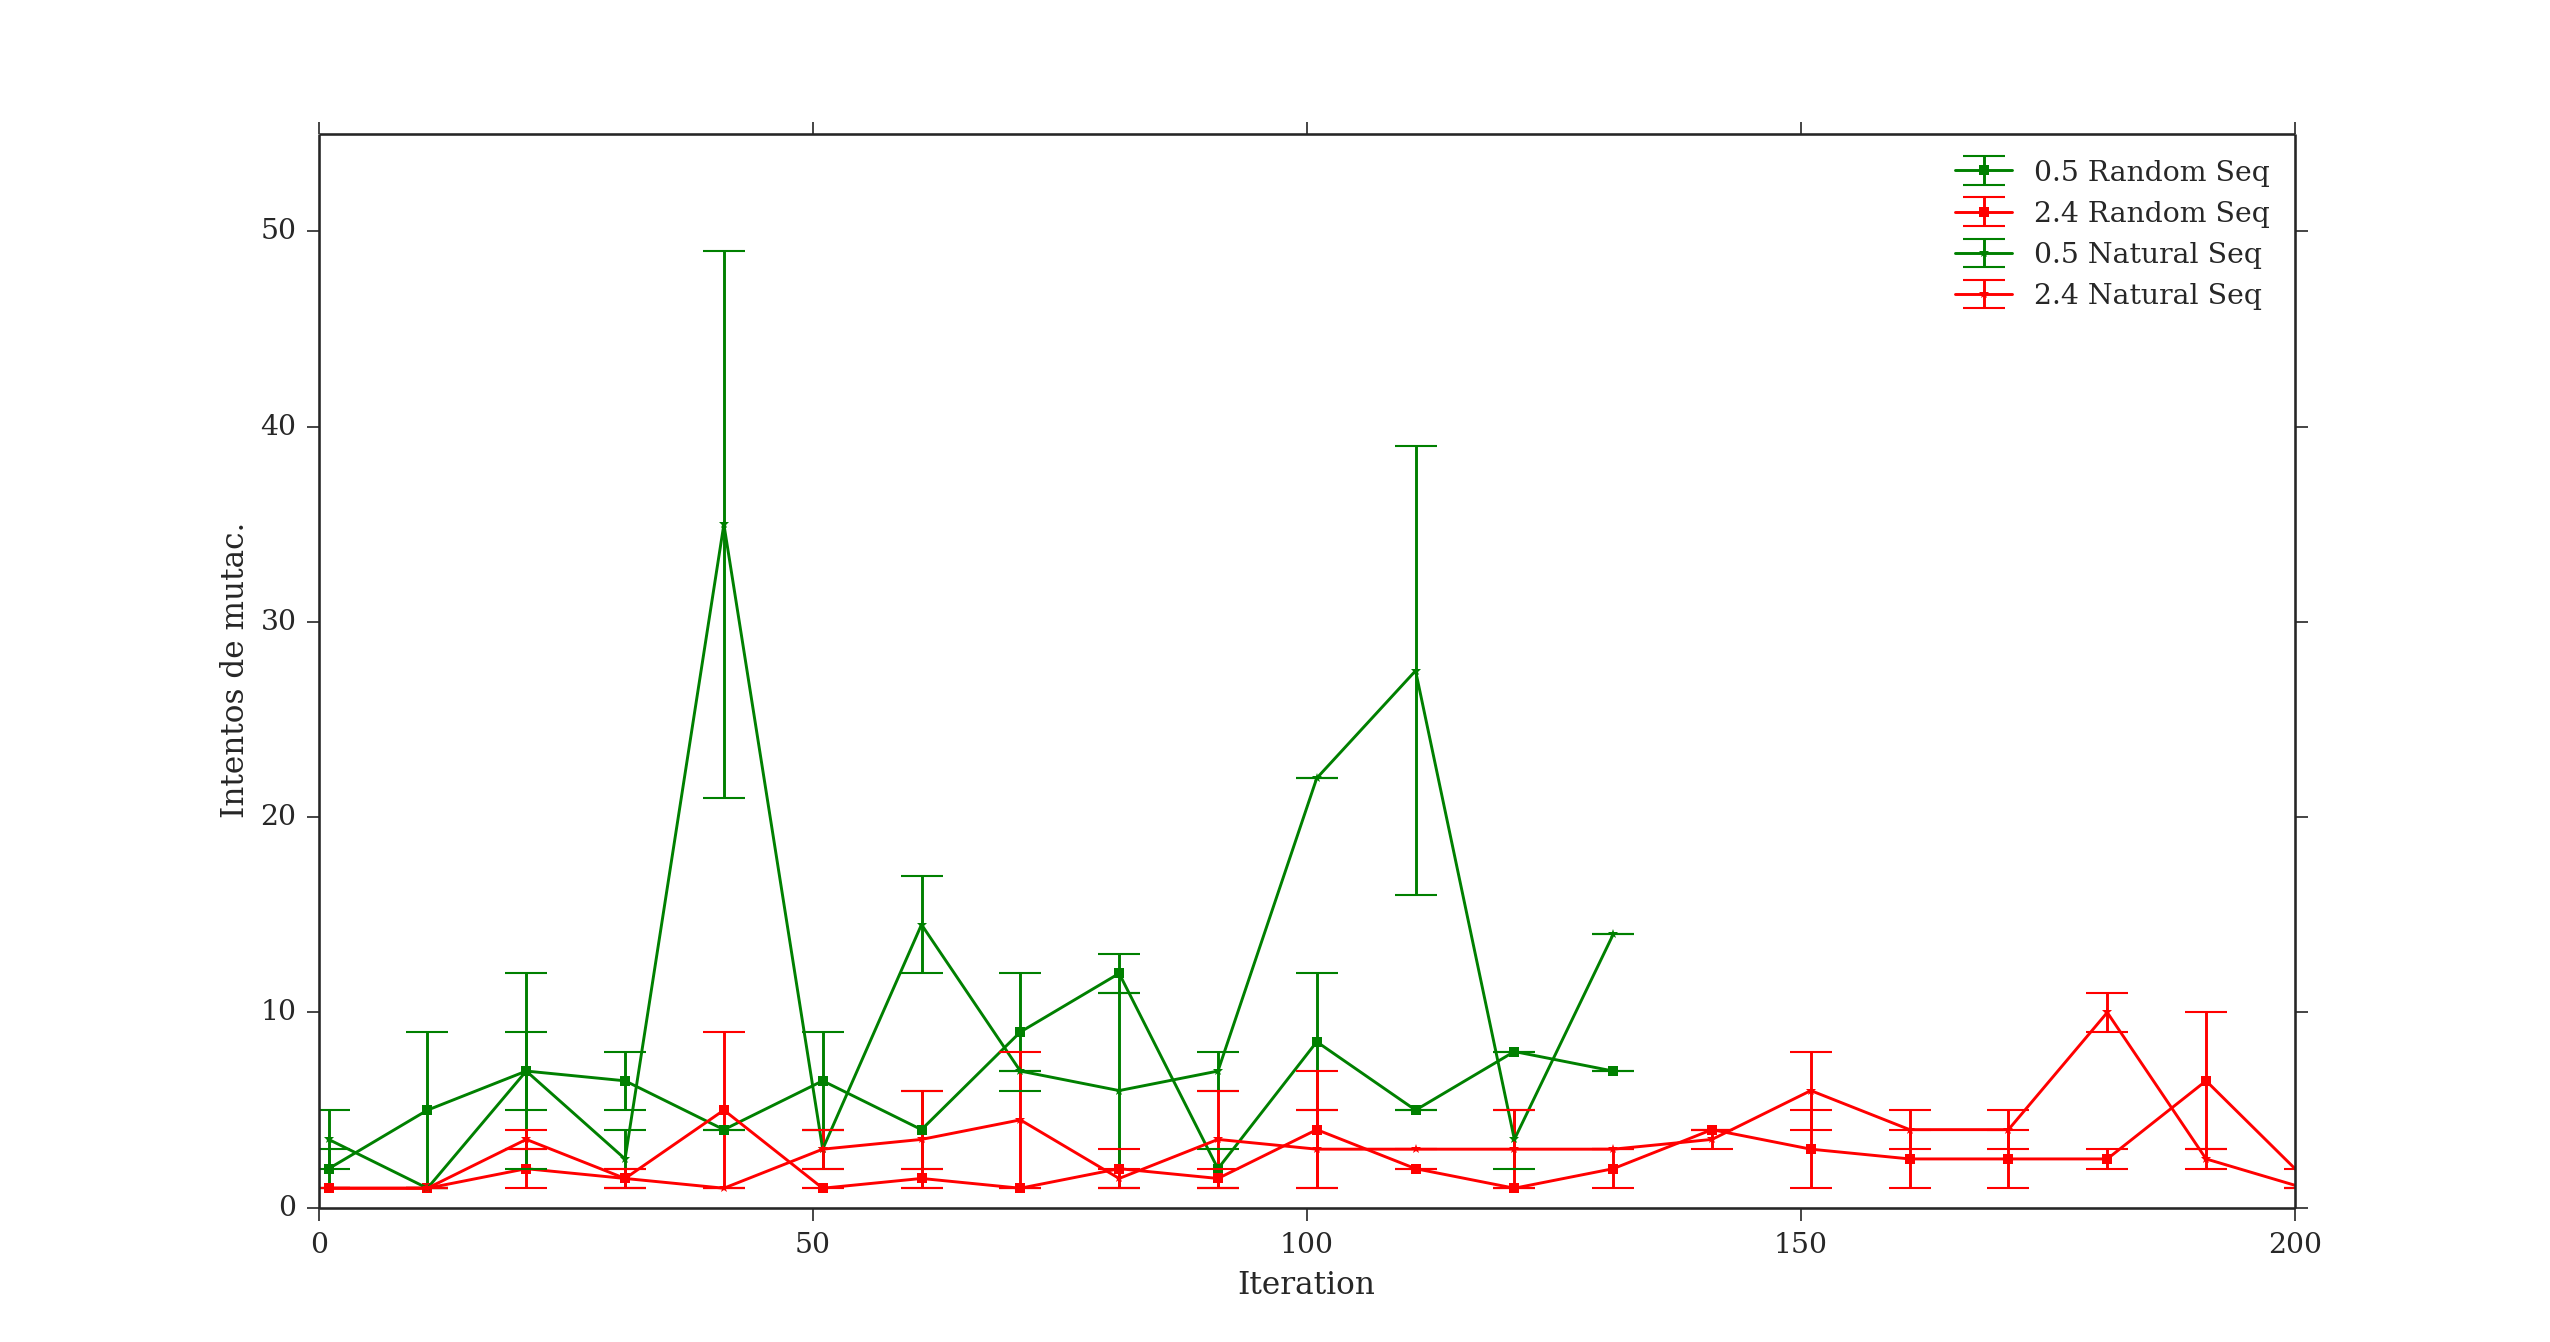
\includegraphics[width=\textwidth,height=0.85\textheight]{mutAttempts.png}
% \end{frame}
% 
% \begin{frame}{Intentos de mutación - Corridas individuales - Seq = 30}
% 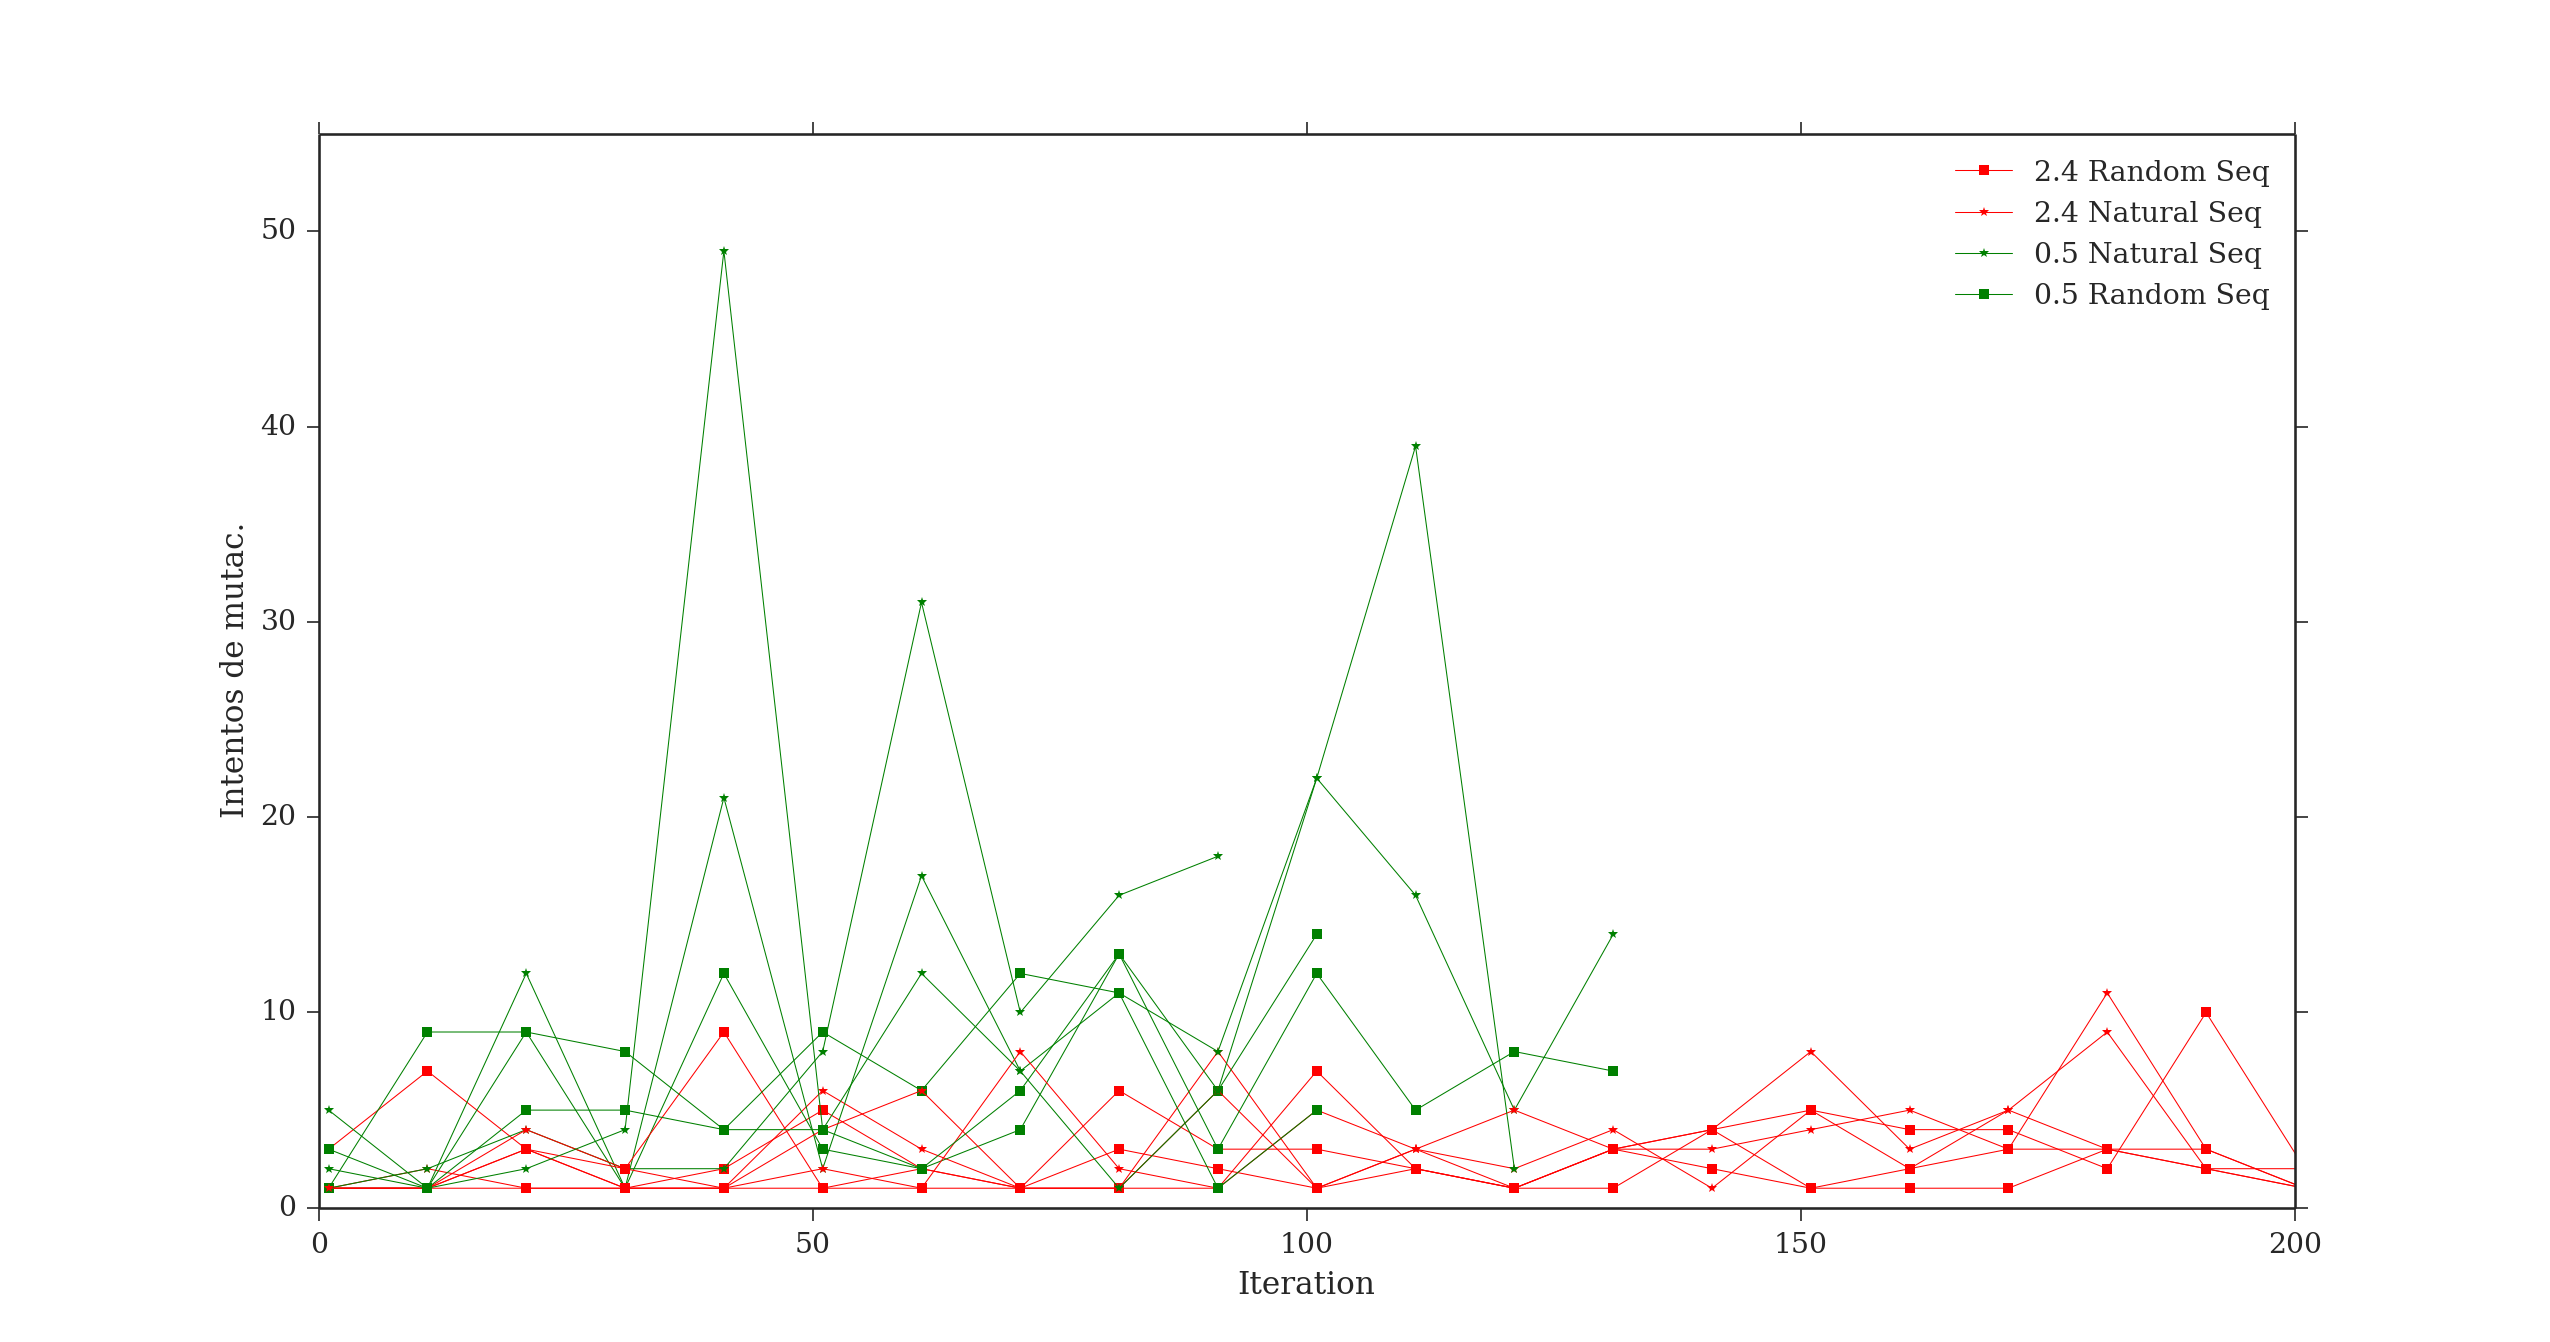
\includegraphics[width=\textwidth,height=0.85\textheight]{mutAttemptsRuns.png}
% \end{frame}
% 
% \begin{frame}{Intentos de mutación - Corridas individuales - Seq = 30}
% 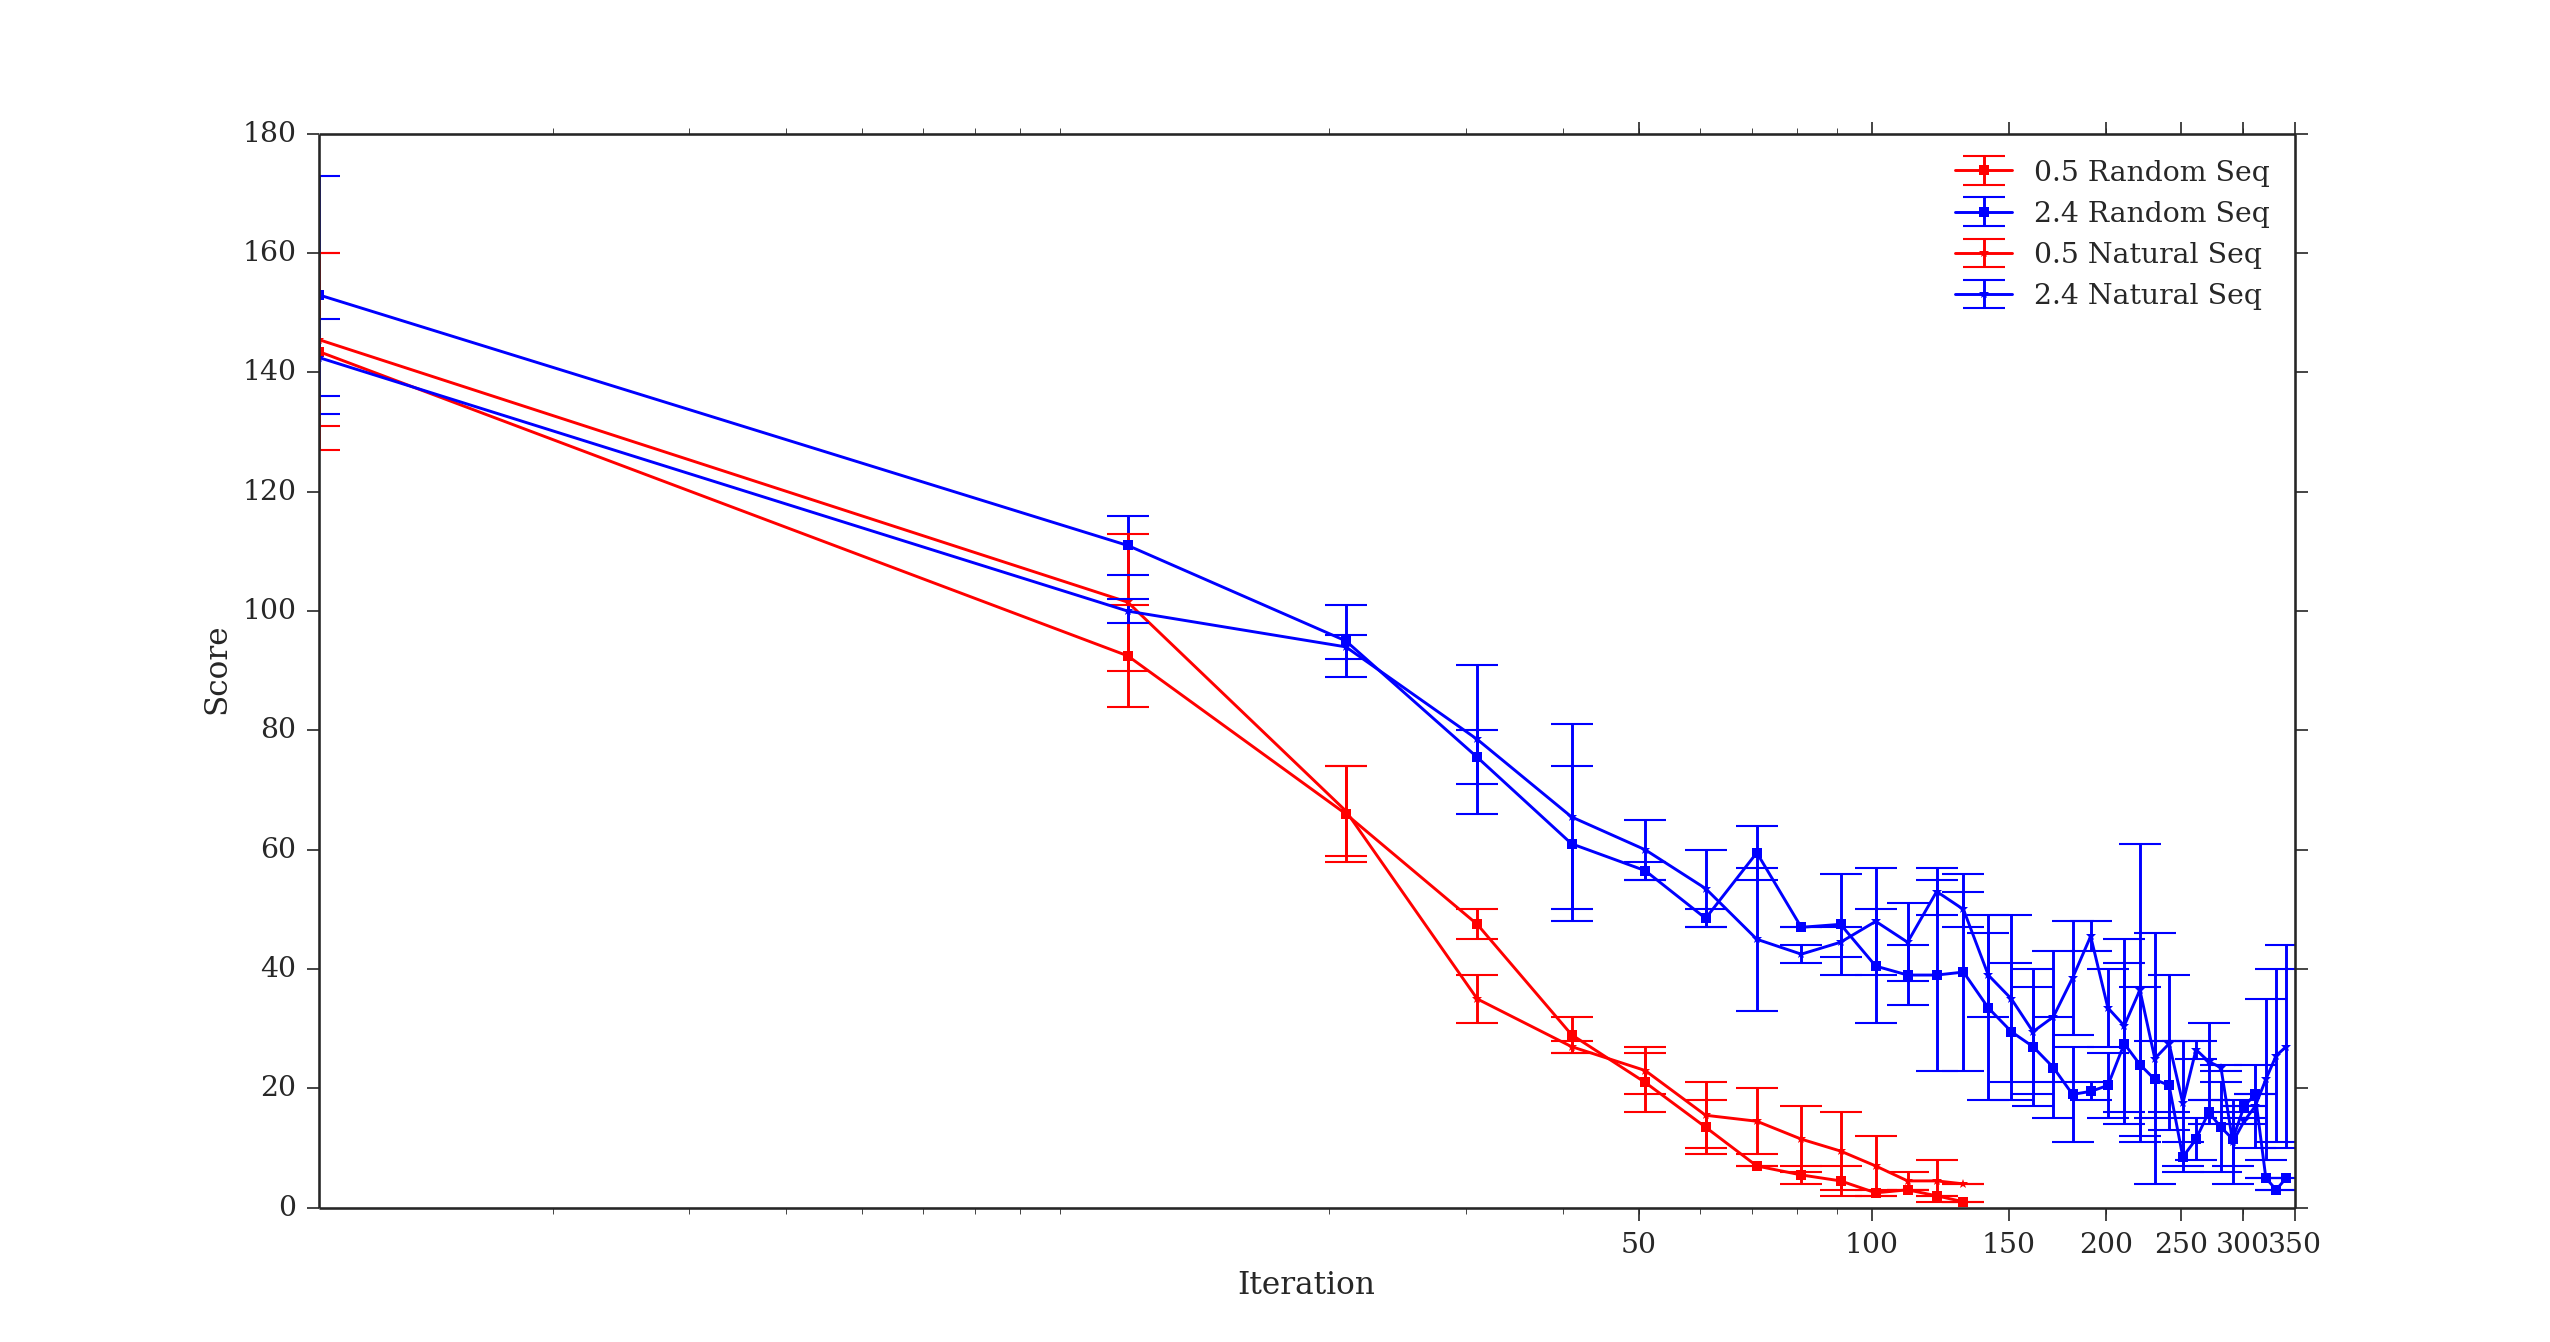
\includegraphics[width=\textwidth,height=0.85\textheight]{scoreVsIterMean.png}
% \end{frame}
% 
% 
% \begin{frame}{Secuencia inicial constante - Divergencia de las ejecuciones}
% 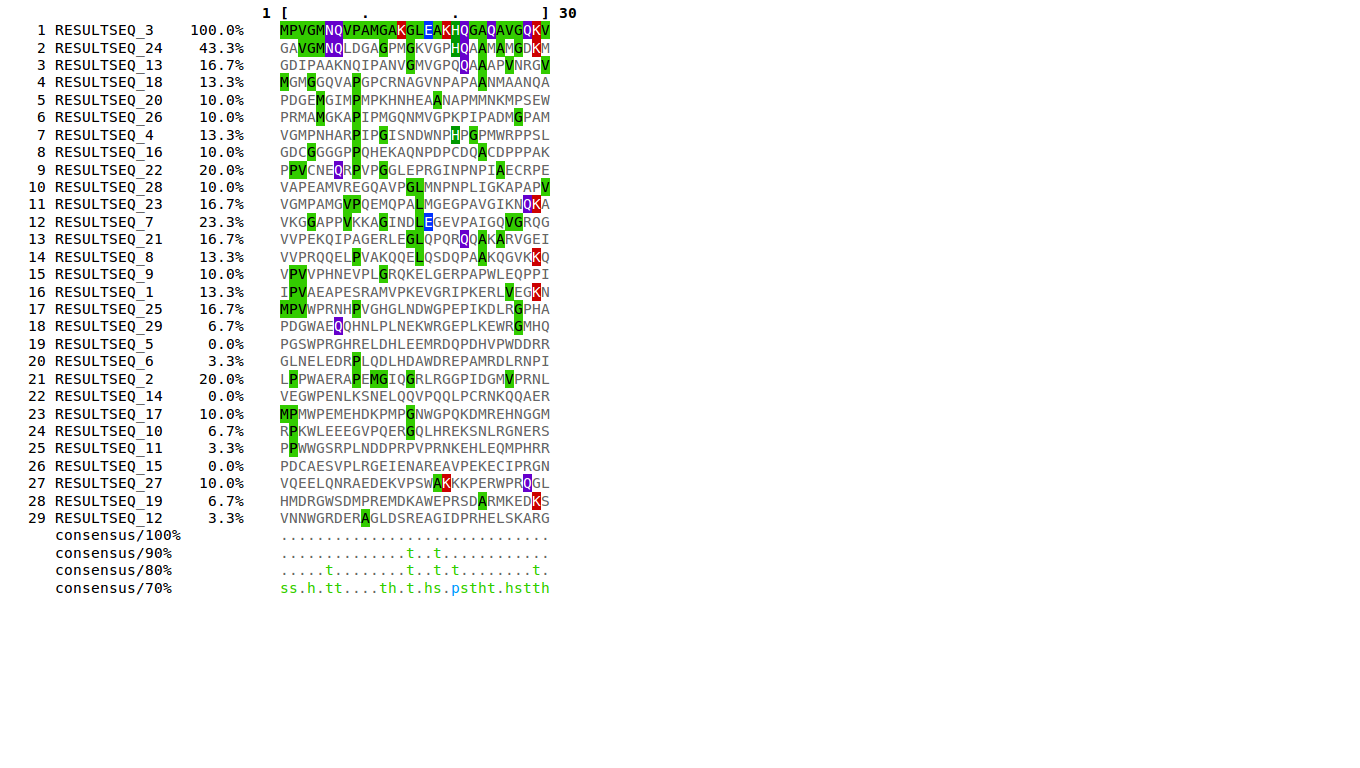
\includegraphics[width=1.5\textwidth,height=1.1\textheight]{divergencia.png}
% \end{frame}

% \section{A futuro}
% 
% \begin{frame}{Queda por hacer}
% \begin{itemize}
% \item Agregar/actualizar herramientas de evaluación, refinar los parámetros de éstas. 
% \item Incorporar las secuencias generadas a una base de datos. 
% %DE ESTA FORMA, DESPUES SE PUEDE ARMAAR UNA FUNCIONALIDAD QUE 
% % ADEMAS, UNA VEZ QUE SE TIENE UNA BD CON UNA CANTIDAD CONSIDERABLE DE SECUENCIAS SE PUEDE  USAR COMO BASE PARA DIFERENTES ESTUDIOS 
% \end{itemize}
% \end{frame}

\end{document}
